\documentclass[11pt]{article}
\usepackage[utf8]{inputenc}	% Para caracteres en español
\usepackage{amsmath,amsthm,amsfonts,amssymb,amscd}
\usepackage{multirow,booktabs}
\usepackage[table]{xcolor}
\usepackage{fullpage}
\usepackage{lastpage}
\usepackage{enumitem}
\usepackage{fancyhdr}
\usepackage{mathrsfs}
\usepackage{wrapfig}
\usepackage{setspace}
\usepackage{calc}
\usepackage{multicol}
\usepackage{cancel}
\usepackage[retainorgcmds]{IEEEtrantools}
\usepackage[margin=1cm]{geometry}
\usepackage{amsmath}
\newlength{\tabcont}
\setlength{\parindent}{0.0in}
\setlength{\parskip}{0.05in}
\usepackage{empheq}
\usepackage{framed}
\usepackage[most]{tcolorbox}
\usepackage{xcolor}
\usepackage{graphicx}
\usepackage{listings}
% -- Basic formatting
\usepackage[utf8]{inputenc}
\usepackage[english]{babel}
\usepackage{times}
\usepackage{caption}
\usepackage{subcaption}
\usepackage{placeins}
\setlength{\parindent}{0pt}
\usepackage{indentfirst}% -- Defining colors:
\usepackage[dvipsnames]{xcolor}
\definecolor{codegreen}{rgb}{0,0.6,0}
\definecolor{codegray}{rgb}{0.5,0.5,0.5}
\definecolor{codepurple}{rgb}{0.58,0,0.82}
\definecolor{backcolour}{rgb}{0.95,0.95,0.92}% Definig a custom style:
\lstdefinestyle{mystyle}{
    backgroundcolor=\color{backcolour},   
    commentstyle=\color{codepurple},
    keywordstyle=\color{NavyBlue},
    numberstyle=\tiny\color{codegray},
    stringstyle=\color{codepurple},
    basicstyle=\ttfamily\footnotesize\bfseries,
    breakatwhitespace=false,         
    breaklines=true,                 
    captionpos=t,                    
    keepspaces=true,                 
    numbers=left,                    
    numbersep=5pt,                  
    showspaces=false,                
    showstringspaces=false,
    showtabs=false,                  
    tabsize=2
}% -- Setting up the custom style:
\lstset{style=mystyle}
\lstset{
  style=mystyle,
  framexleftmargin=3.5mm,
  rulesepcolor=\color{black},
  linewidth=0.6\linewidth,
  xleftmargin=12pt,
  aboveskip=12pt,
  belowskip=12pt
}
\colorlet{shadecolor}{orange!15}
\parindent 0in
\parskip 1pt
\geometry{margin=1in, headsep=0.25in}
\theoremstyle{definition}
\newtheorem{defn}{Definition}
\newtheorem{reg}{Rule}
\newtheorem{exer}{Exercise}
\newtheorem{note}{Note}
\graphicspath{ {./images/} }
\begin{document}
\setcounter{section}{0}
\title{MIE223 Lecture Notes}

\thispagestyle{empty}

\begin{center}
{\LARGE \bf Introduction to Bayesian Data Analysis}\\
{\large MIE223}\\
Winter 2025
\end{center}
\section{Bayesian Data Analysis}

\subsection{Bayesian Motivation: Bayesian Decision Theory}
\begin{itemize}
    \item Robot has belief P(x|D) over position
    \begin{itemize}
        \item D consists of noisy range finder readings
    \end{itemize}
    \item Associate Risk(x) w\ position x (e.g., stairs!)
    \begin{itemize}
        \item MAP Risk = Risk(x*) = 0 (Max Posterior)
        \item E(p(x|d))(Risk(x))
        \item Full Bayesian Risk = x Risk(x)p(x|D) > 0
    \end{itemize}
    \item Which risk estimate would you use?
\end{itemize}

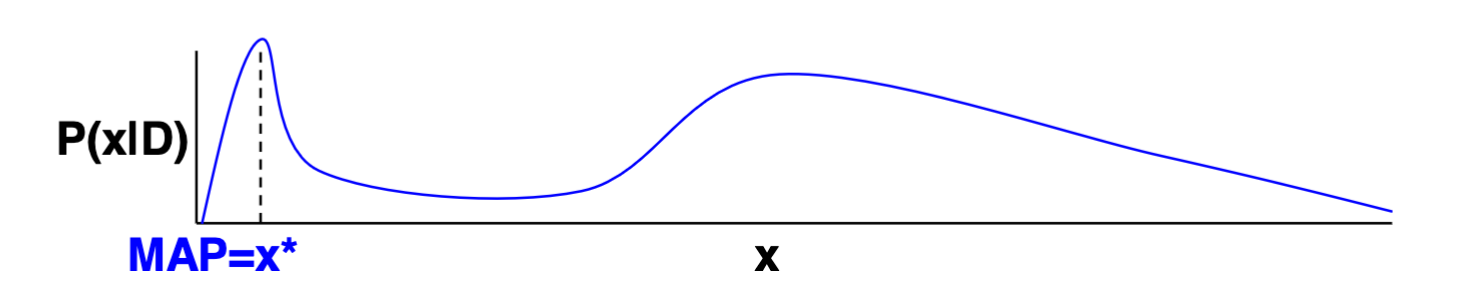
\includegraphics[width=\textwidth/2-2.08049pt]{1.png}
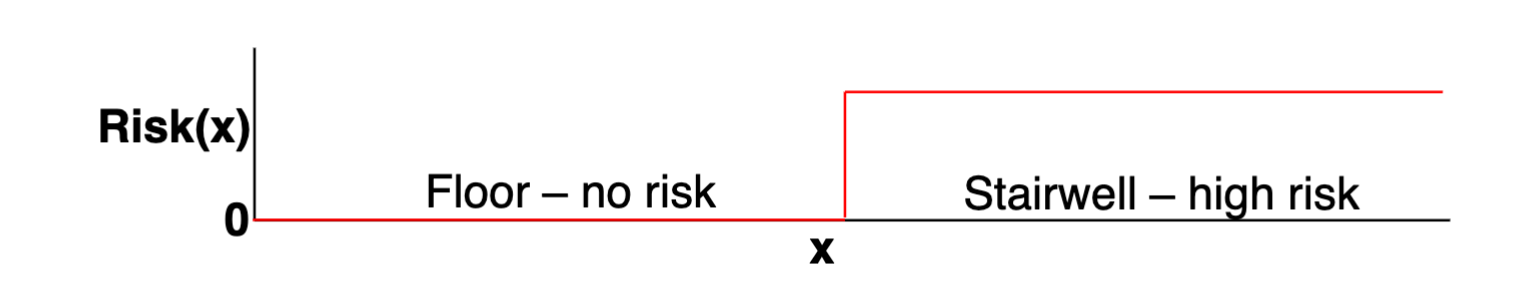
\includegraphics[width=\textwidth/2]{2.png}

\subsection{Bayesian Generative View of Data}
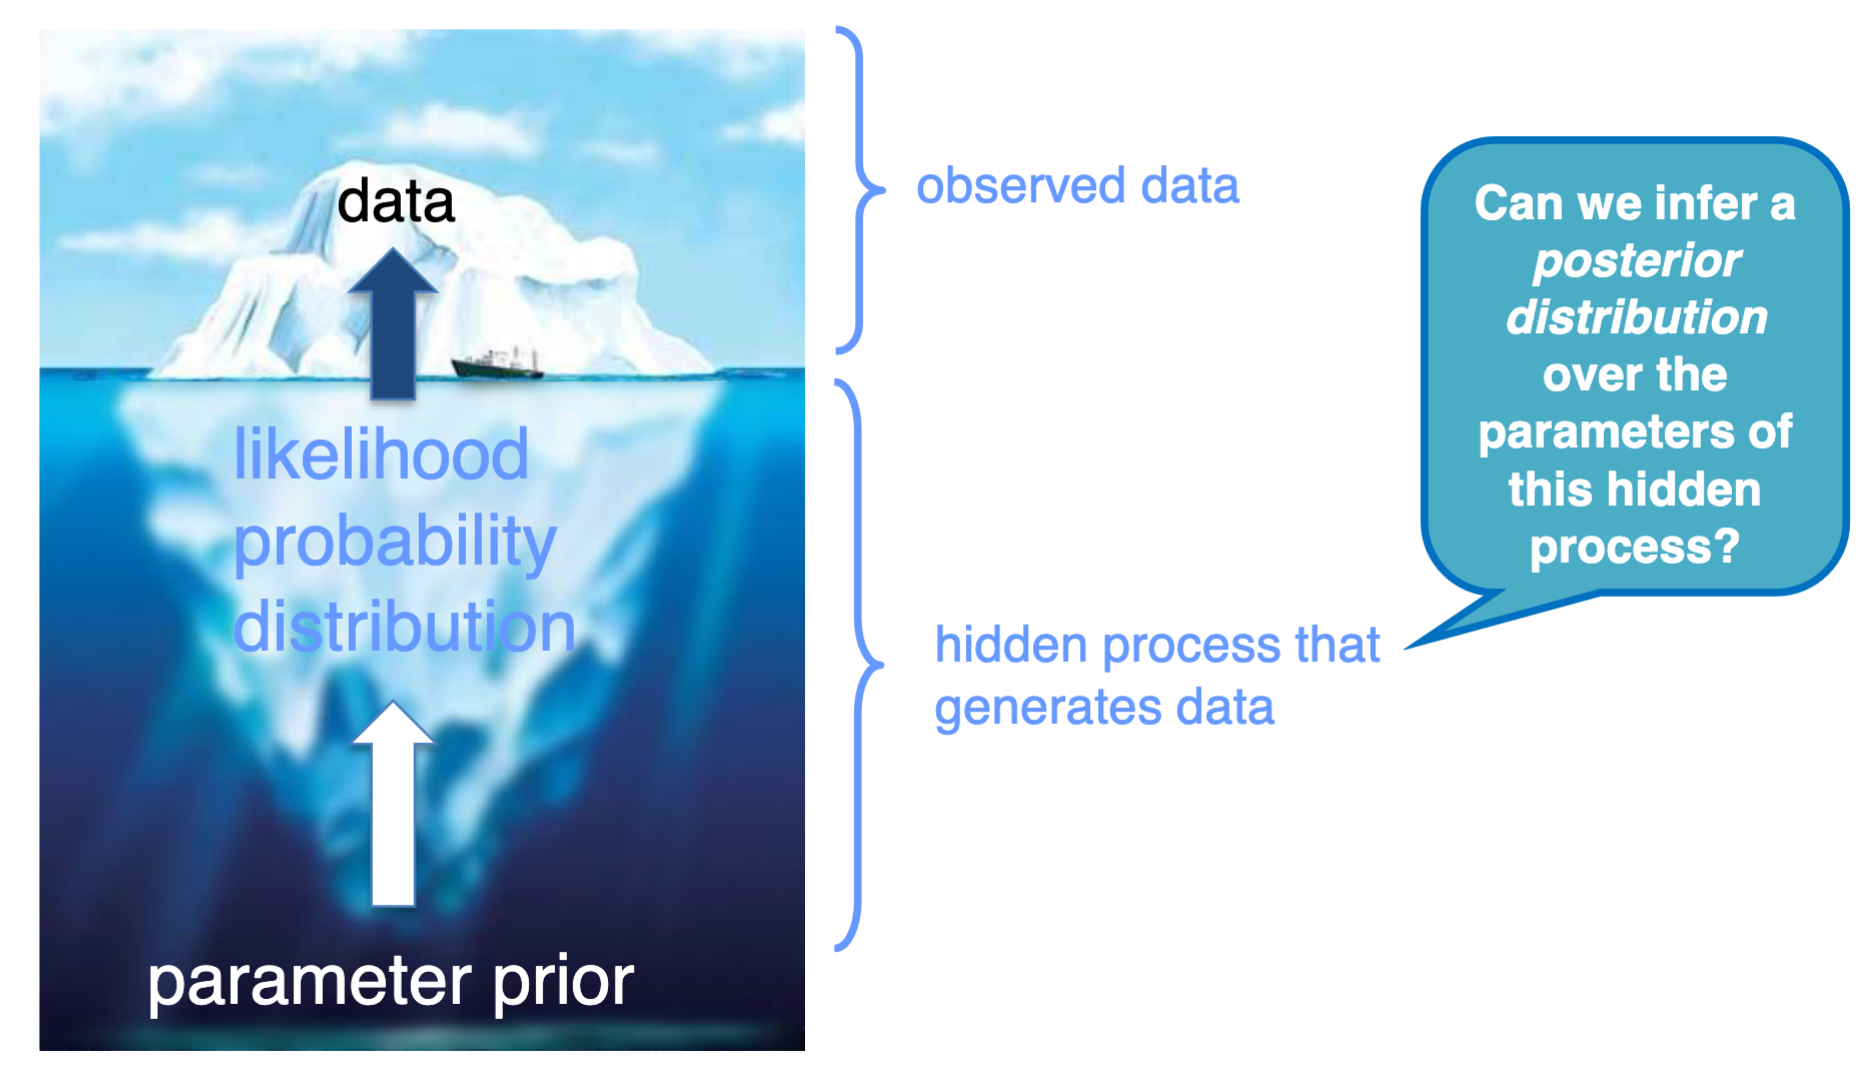
\includegraphics[width=\textwidth/2]{3.png}

\subsection{A coin tossing example}
\begin{itemize}
    \item Suppose we know nothing about coins except that each tossing
    event produces a head with some unknown probability p and a
    tail with probability 1-p.
    \begin{itemize}
        \item Our model of a coin has one parameter, p.
    \end{itemize}
    \item If we observe 1 heads in 1 toss, what is p?
    \item If we observe 5 heads in 10 tosses, what is p?
    \item If we observe 53 heads in 100 tosses, what is p?
    \begin{itemize}
        \item How confident are we in each case?
    \end{itemize}
    \item The frequentist answer (also called maximum likelihood):
    Pick the value of p that makes the observation of 53 heads and
    47 tails most probable.
    \begin{itemize}
        \item This value is p=0.53
    \end{itemize}
\end{itemize}

\subsection{A coin tossing example: maximum likelihood (frequentist estimation)}
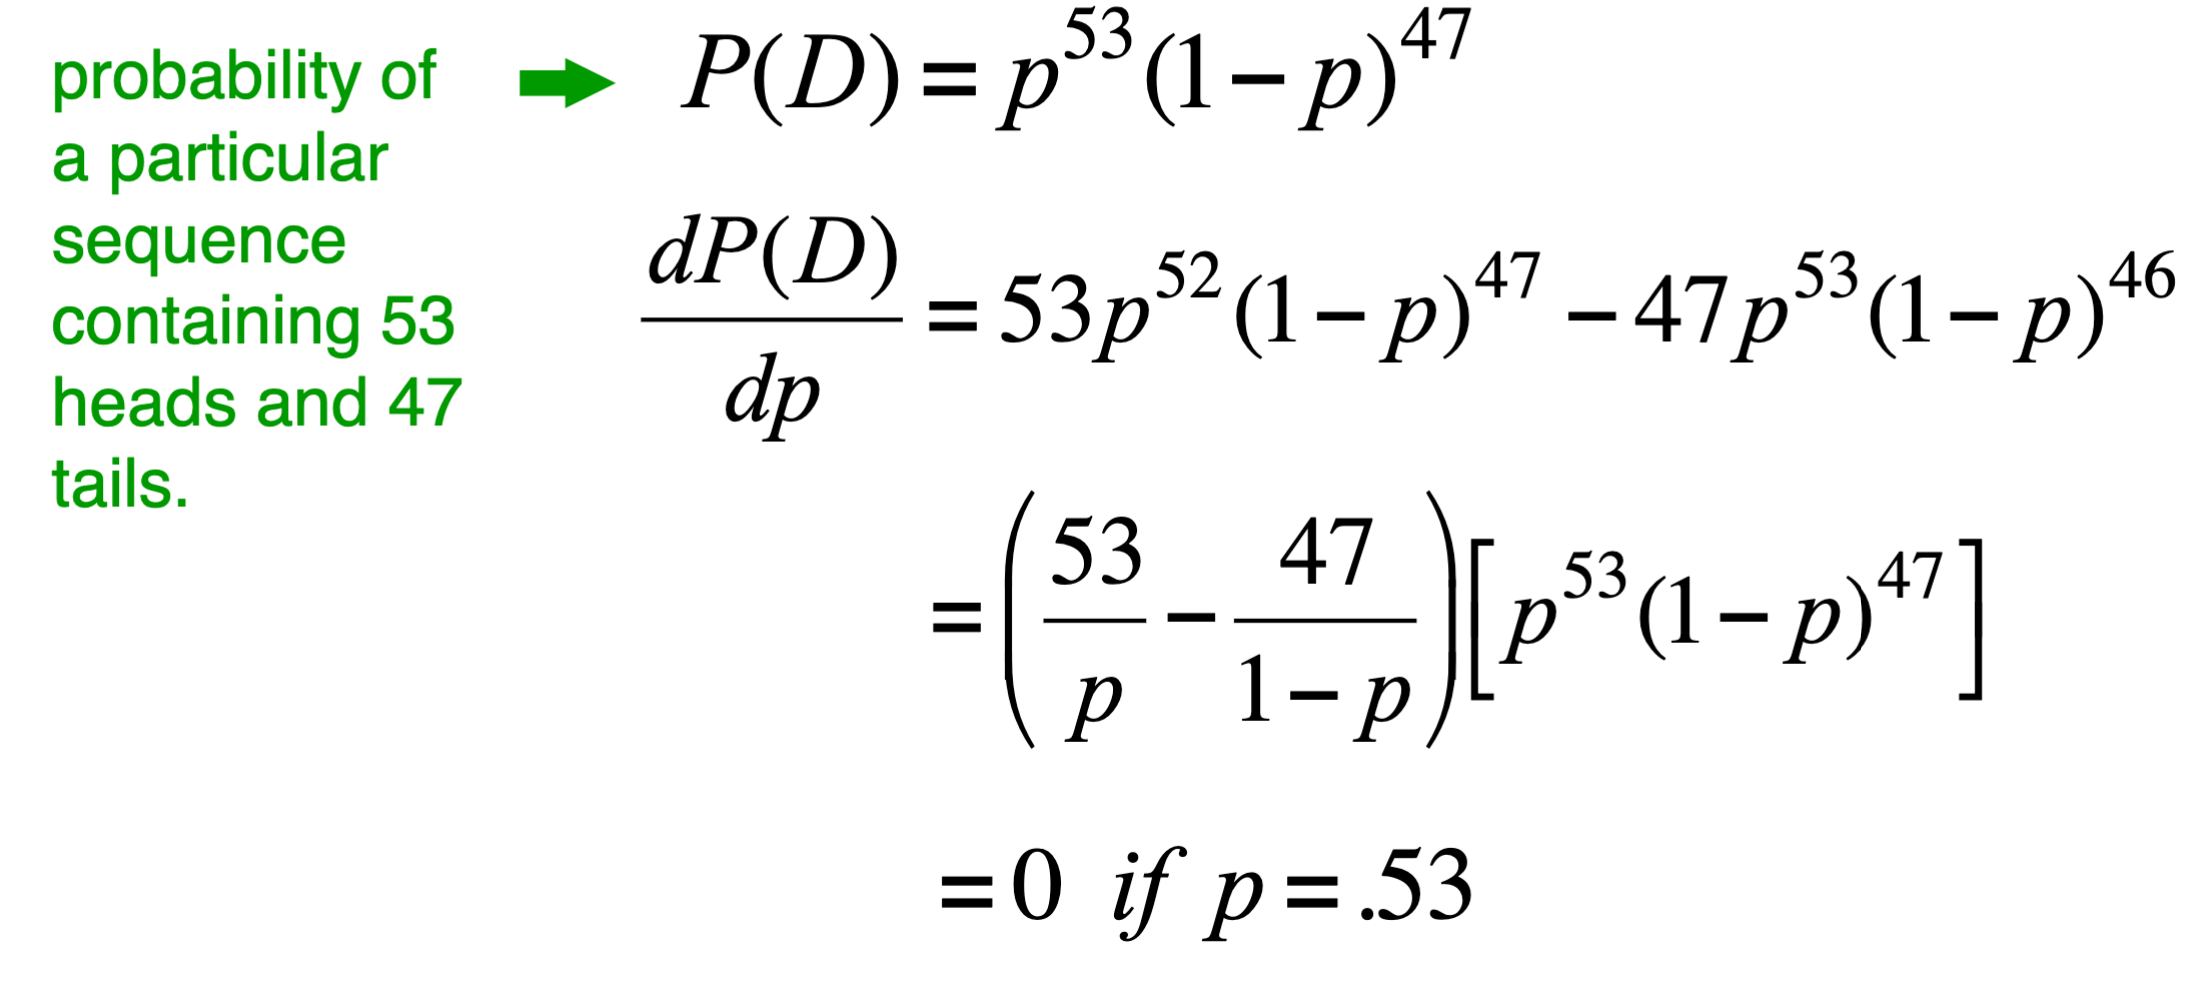
\includegraphics[width=\textwidth/2]{4.png}

\subsection{Some problems with picking the parameters that
are most likely to generate the data}
\begin{itemize}
    \item What if we only
    tossed the coin once
    and we got 1 head?
    \begin{itemize}
        \item Is p=1 a sensible
        answer?
        \item Surely p=0.5 is a
        much better
        answer.
    \end{itemize}
    \item Is it reasonable to give a single
    answer?
    \begin{itemize}
        \item If we don’t have much data,
        we are unsure about p.
        \item Our computations of
        probabilities will work much
        better if we take this
        uncertainty into account.
    \end{itemize}
\end{itemize}

\subsection{The Bayesian Perspective}
\begin{itemize}
    \item Rather than taking the
    most likely estimate of p
    (i.e. maximum
    likelihood)...
    \item Let’s build a Bayesian
    posterior distribution
    over our belief in p
    \item The more data we see,
    the more “peaked” our
    belief in the correct
    value of p
\end{itemize}

\subsection{Generative Graphical Model for Biased Coin}

\begin{itemize}
    \item We have one latent parameter \( p \)
    \begin{itemize}
        \item With a prior distribution (Beta)
    \end{itemize}
    \item Generates data via a likelihood
    \begin{itemize}
        \item With a Bernoulli distribution
    \end{itemize}
    \item Infer posterior distribution
    \begin{itemize}
        \item Also Beta since this is a conjugate prior-posterior pair
    \end{itemize}
\end{itemize}

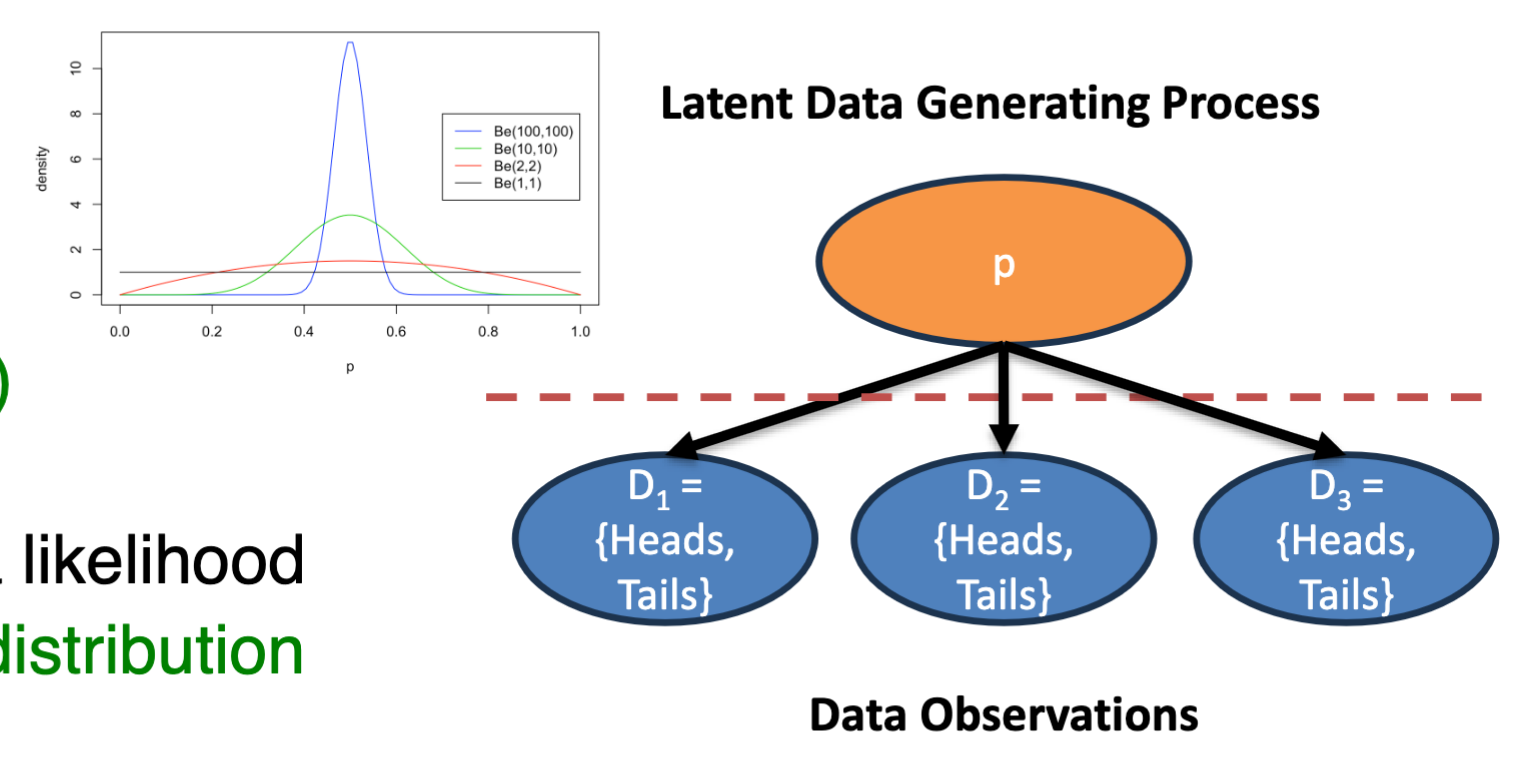
\includegraphics[width=\textwidth/2]{9.png}

How likely is HTH given p? p(1-p)p.

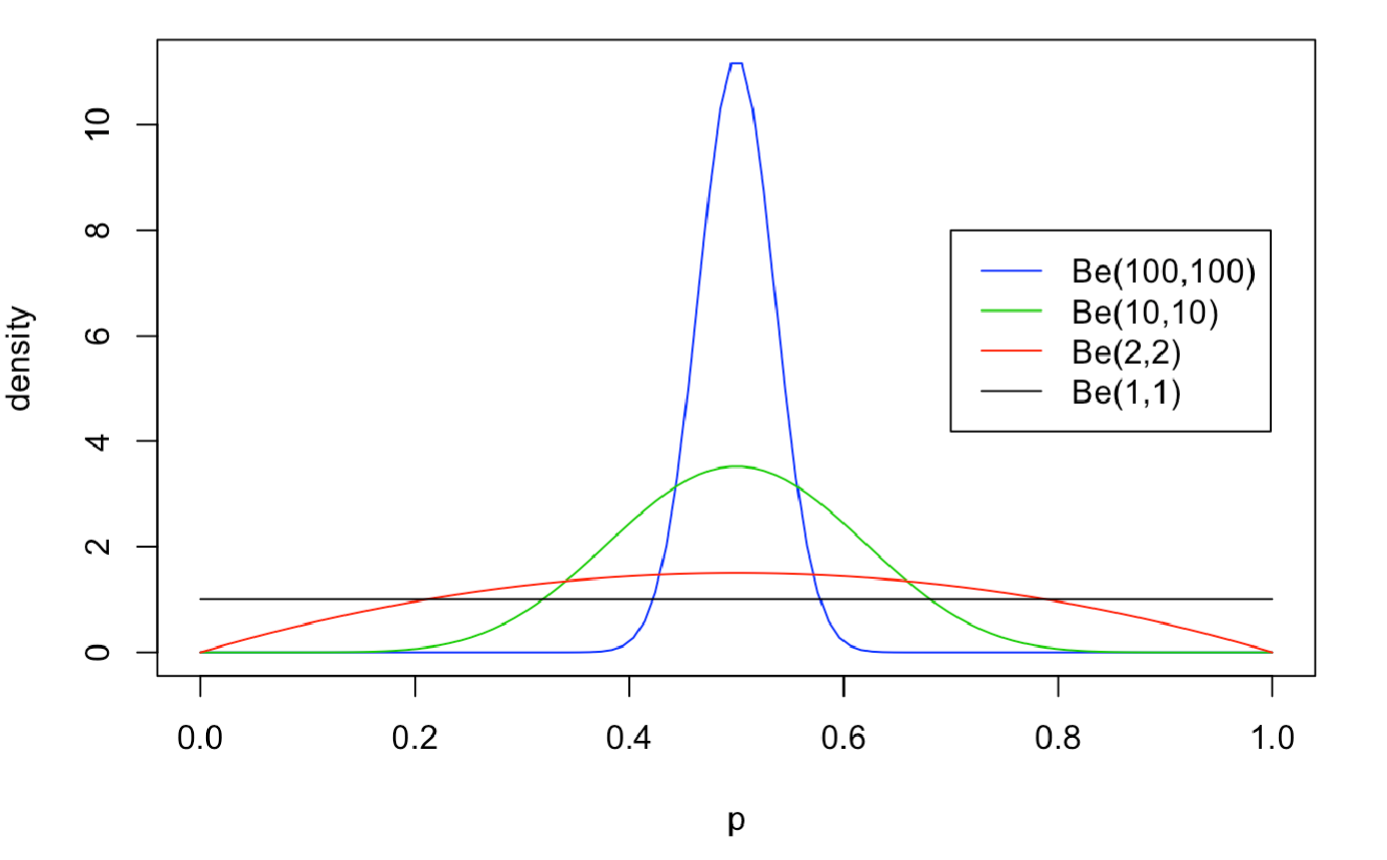
\includegraphics[width=\textwidth/2]{5.png}

\subsection{Using a distribution over parameter values}
\begin{itemize}
    \item Start with a prior distribution over
    p. In this case we used a uniform
    distribution.
    \item Multiply the prior probability of
    each parameter value by the
    probability of observing a head
    given that value (likelihood).
    \item Then scale up all of the probability
    densities so that their integral
    comes to 1. This gives the
    posterior distribution.
\end{itemize}


\subsection{Lets do it again: Suppose we get a tail}
\begin{itemize}
    \item Start with a prior distribution
    over p.
    \item Multiply the prior probability
    of each parameter value by
    the probability of observing
    a tail given that value.
    \item Then renormalize to get the
    posterior distribution. Look
    how sensible it is!
\end{itemize}

\subsection{Lets do it another 98 times}

\begin{itemize}
    \item After 53 heads and 47
    tails we get a very
    sensible posterior
    distribution that has its
    peak at 0.53 (assuming a
    uniform prior)
\end{itemize}

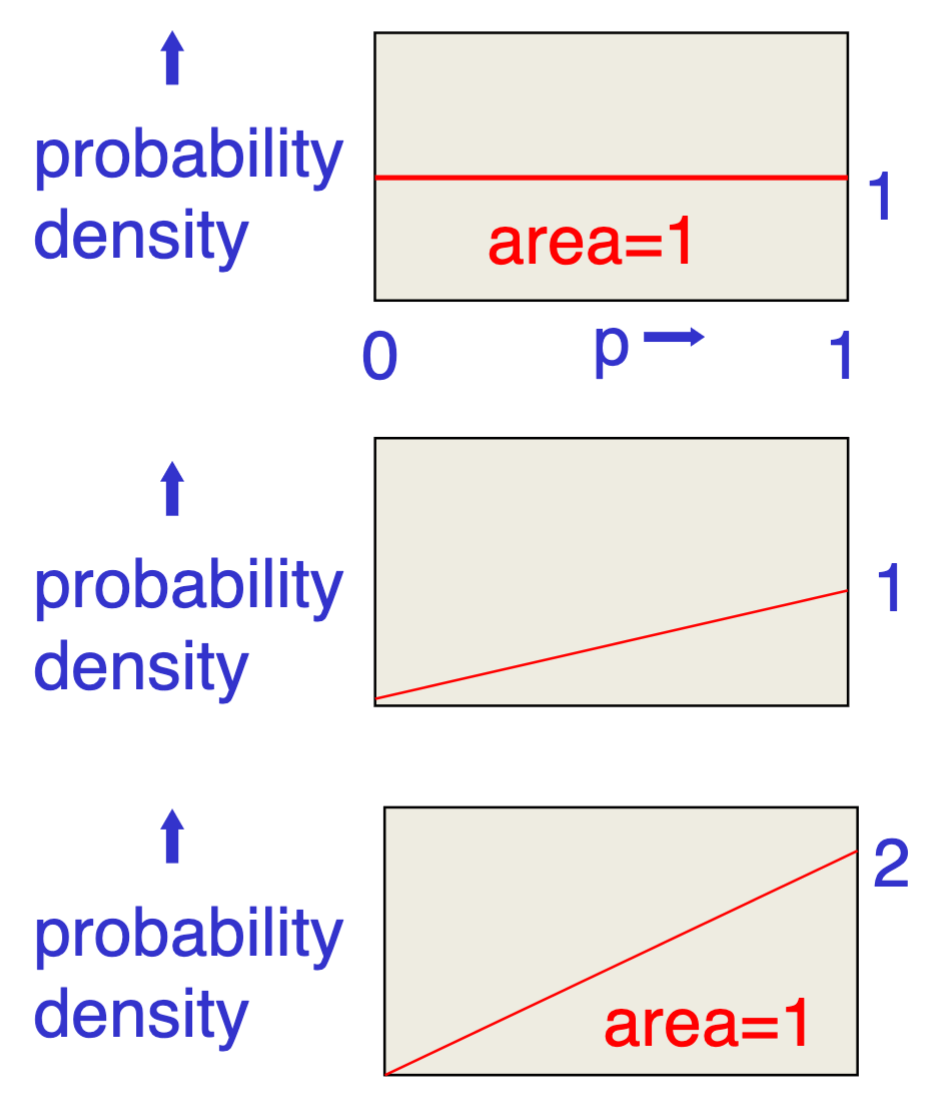
\includegraphics[width=\textwidth/3-4.16101pt]{6.png}
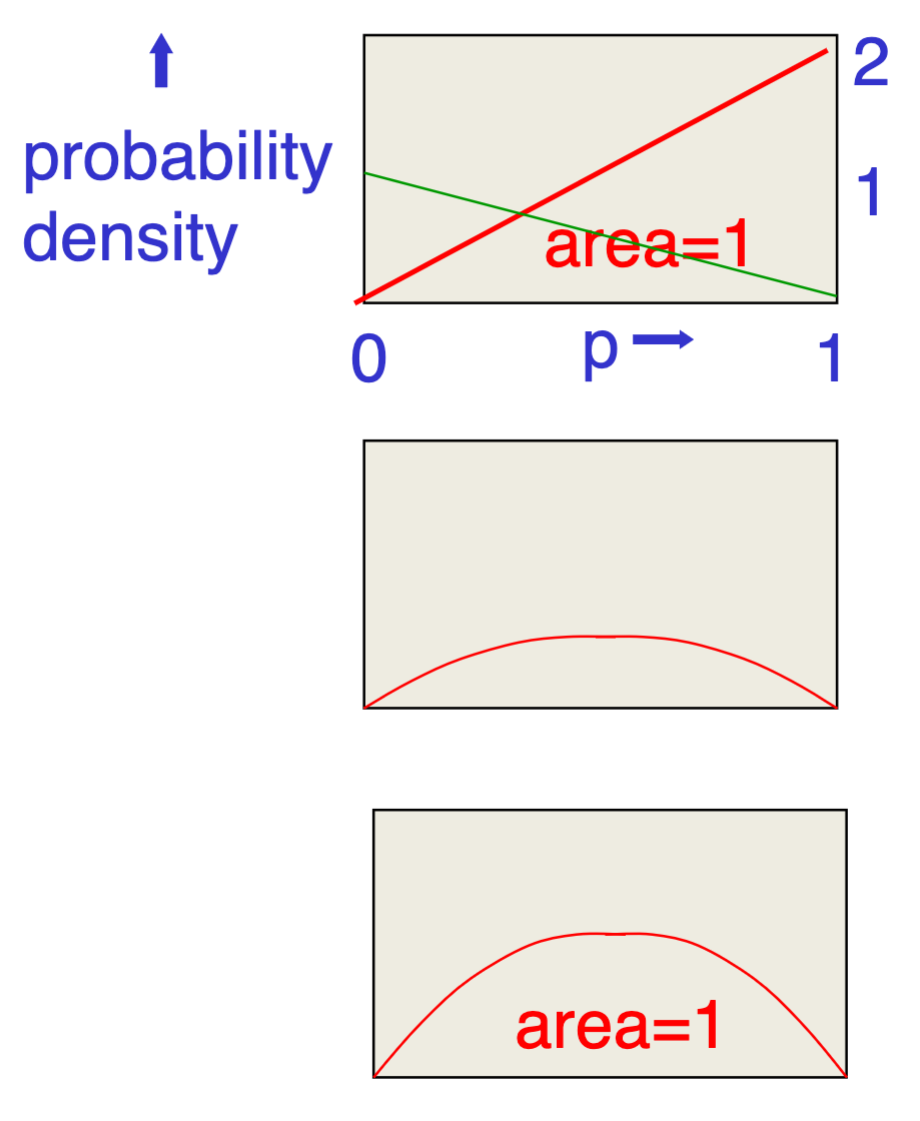
\includegraphics[width=\textwidth/3]{7.png}
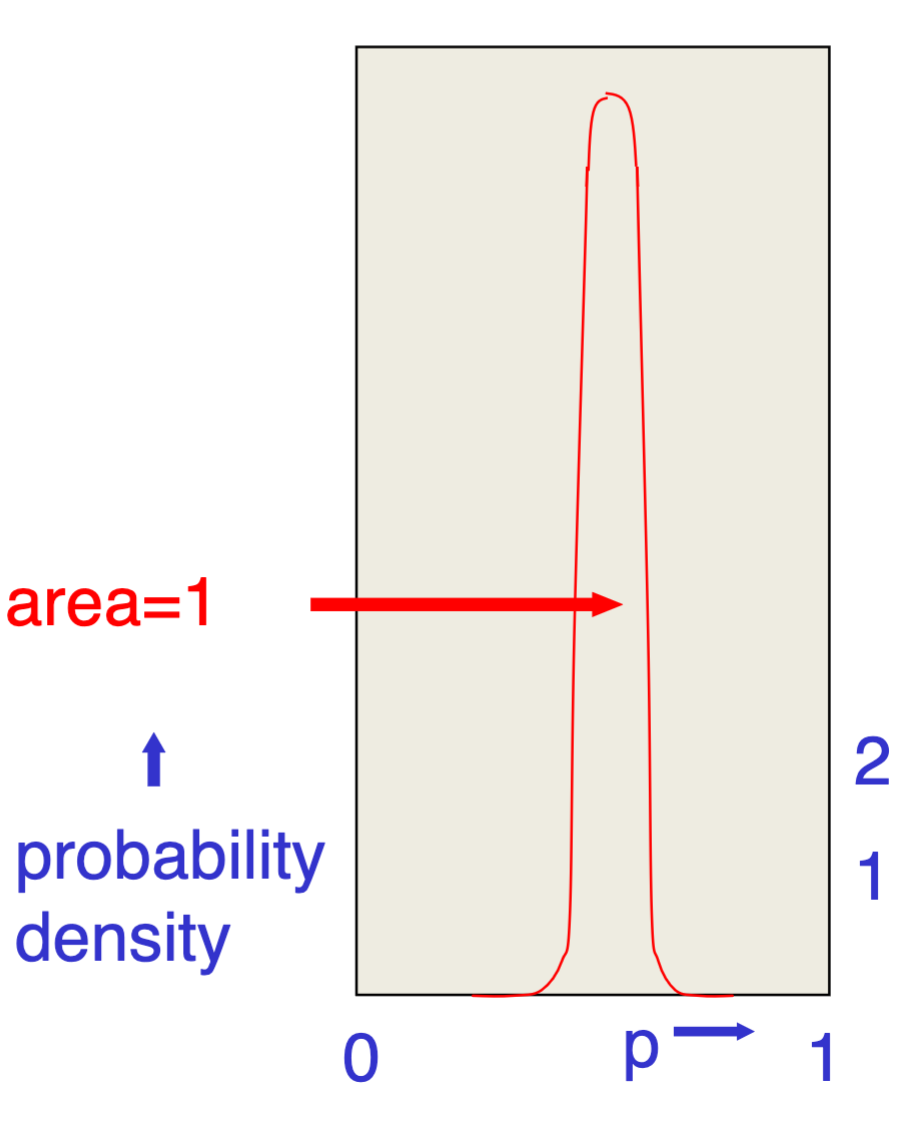
\includegraphics[width=\textwidth/3]{8.png}

\subsection{Bayes Theorem}
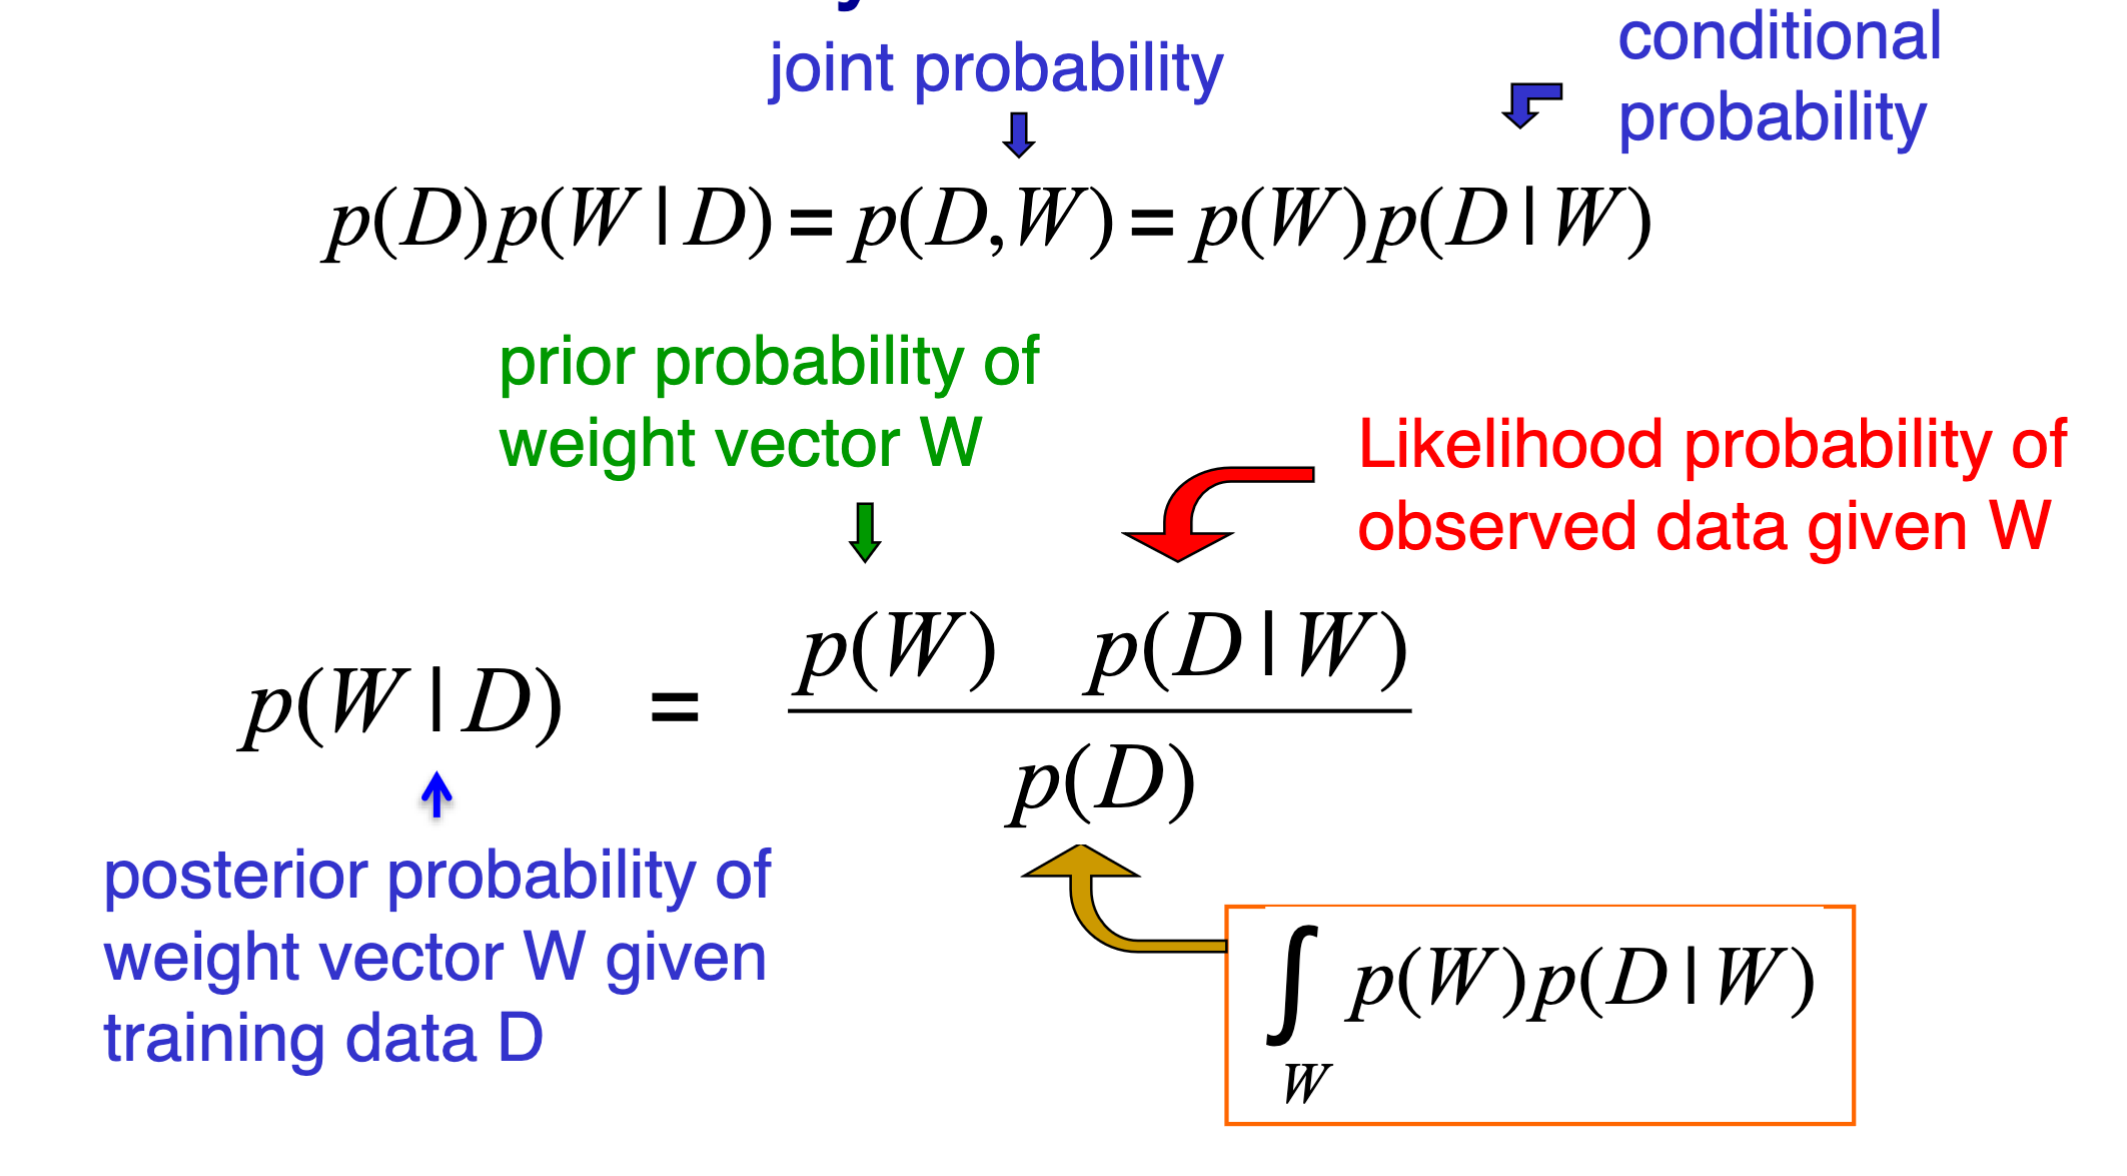
\includegraphics[width=\textwidth/2]{10.png}

\subsection{Aside: Bayesian Graphical Model Notation}
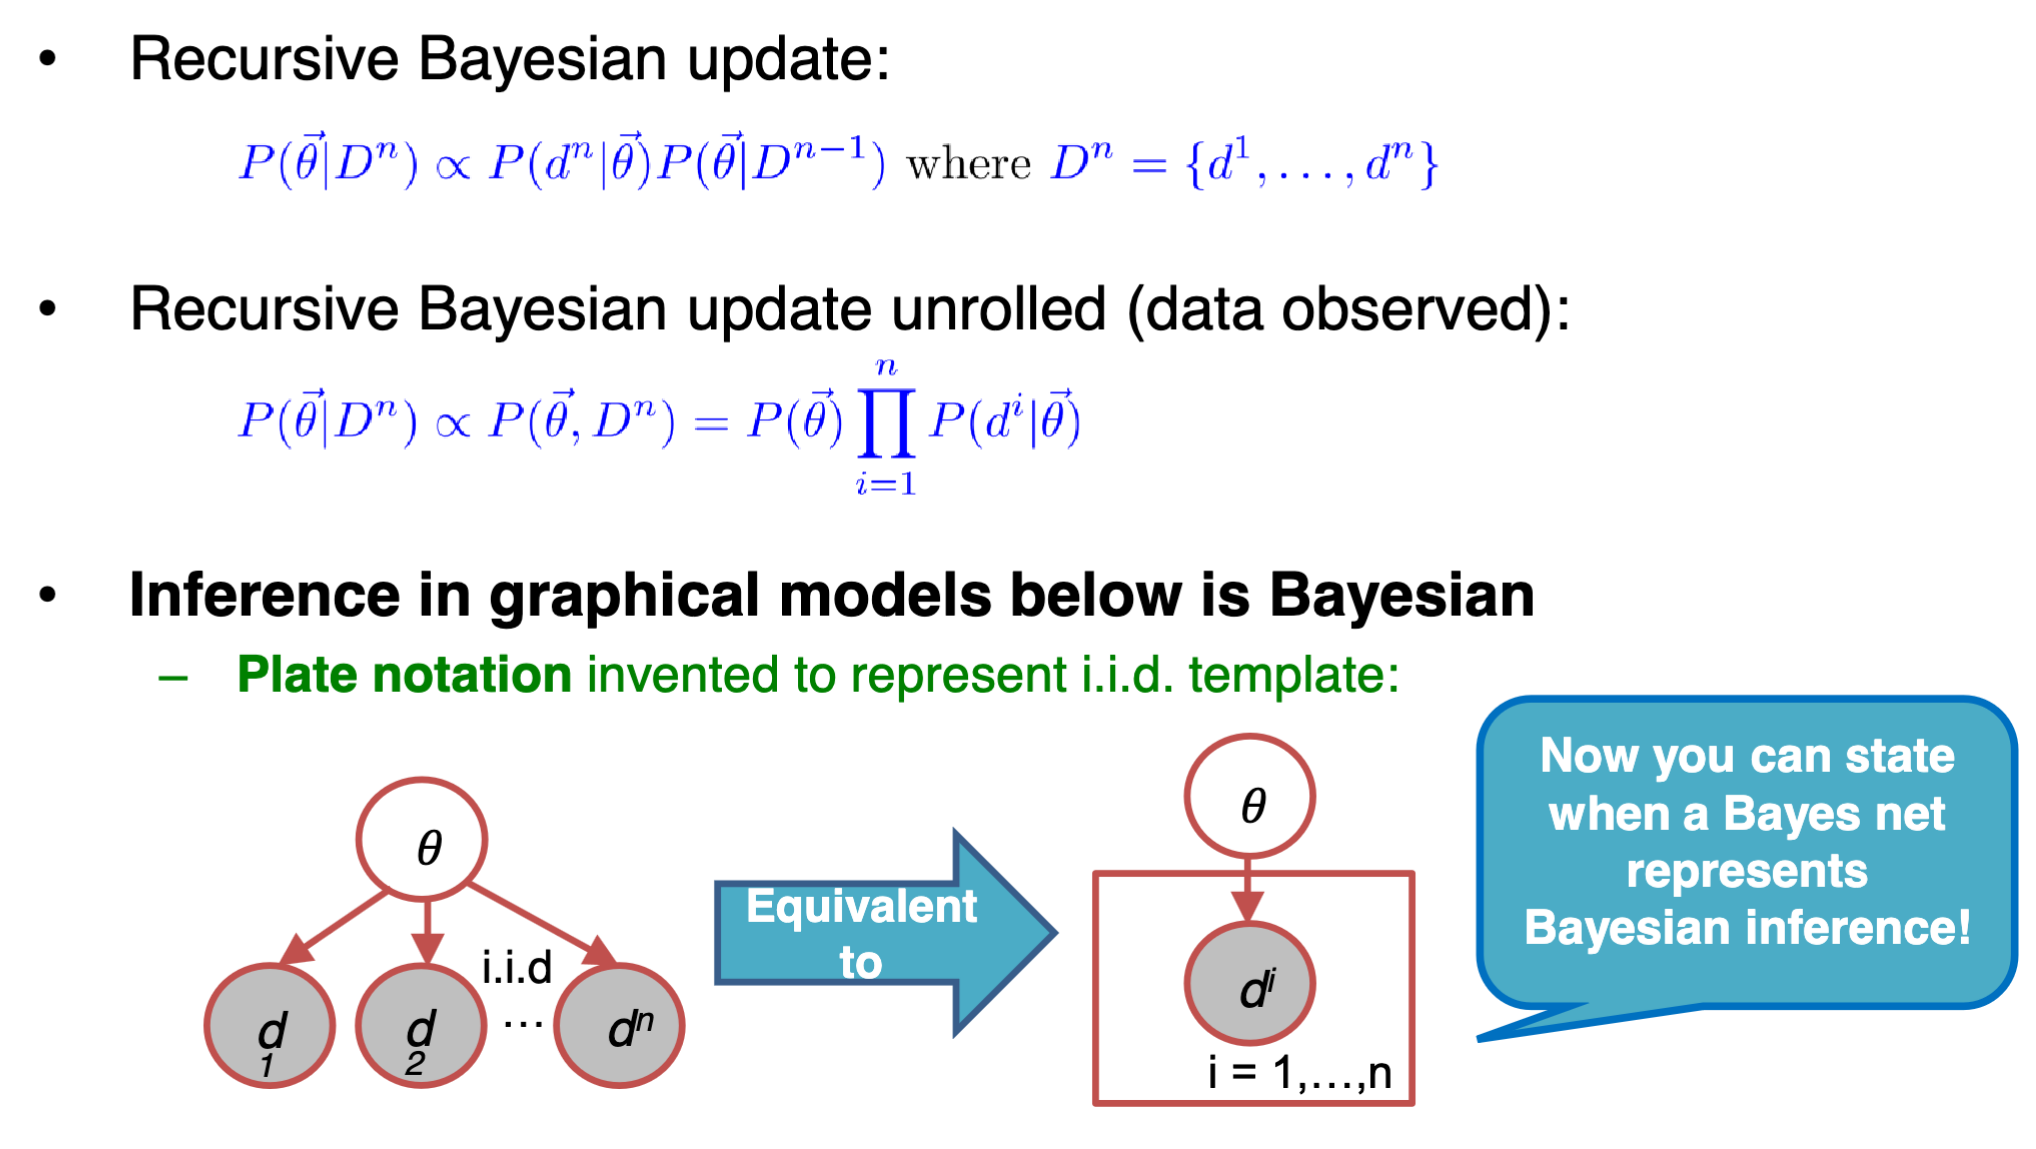
\includegraphics[width=\textwidth/2]{11.png}

bernoulli processes are iid.

\subsection{Sanner on the Chalkboard}

\begin{equation}
    P(A|B) = \frac{P(B|A)P(A)}{P(B)}
\end{equation}

It's proportional to P(B $\vert$ A)P(A) because P(B) is a constant.

posterior is proportional to likelihood times prior.

proportional to:

\begin{equation}
    \prod_{i=1}^{n} P(x_i|\theta)P(\theta)
\end{equation}

\[
P(p) =
\begin{cases} 
1 & \text{if } 0 \leq p \leq 1 \\
0 & \text{otherwise}
\end{cases}
\]

P(D$_1$ = Head$|$p) = p

With enough data, the dirac delta function will peak at the true value of p.
It also happens to be the maximum likelihood estimate.

\subsection{Why Bayesian Data Analysis? Sparse Data}
\begin{itemize}
    \item Choropleth at
    right shows
    countries with
    lowest 10\% death
    rates for kidney
    cancer
    \item Should we live in
    the Midwest to
    avoid kidney
    cancer?
    \item What went
    wrong? Small data due to small populations.
    A lot of people just don't get kidney cancer.
    We come up with a prior distribution.
    Then we can update our local beliefs based on the data.
\end{itemize}


\includegraphics[width=\textwidth/2]{13.png}

\subsection{Why Bayesian Data Analysis? Small Data}

\begin{itemize}
    \item Why Bayesian? Small Data. (Gelman, 2005)
    \begin{itemize}
        \item Sample sizes are never large.
        \item If N is too small to get a sufficiently-precise estimate, you need to get more
        data (or make more assumptions).
        \item But once N is "large enough”, you can start subdividing the data to learn
        more (for example, in a public opinion poll, once you have a good estimate
        for the entire country, you can estimate among men and women,
        northerners and southerners, different age groups, etc.).
        \item N is never enough because if it were "enough" you'd already be on to the
        next problem for which you need more data.
    \end{itemize}
\end{itemize}

\subsection{The Bayesian framework}

The Bayesian framework assumes that we always have a prior
distribution for everything.

\begin{itemize}
    \item The prior may be very vague.
    \item When we see some data, we combine our prior distribution
    with a likelihood term to get a posterior distribution.
    \item The likelihood term takes into account how probable the
    observed data is given the parameters of the model.
    \begin{itemize}
        \item It favors parameter settings that make the data likely.
        \item It fights the prior
        \item With enough data the likelihood terms always wins.
    \end{itemize}
\end{itemize}

\subsection{A More Complex Generative Process}
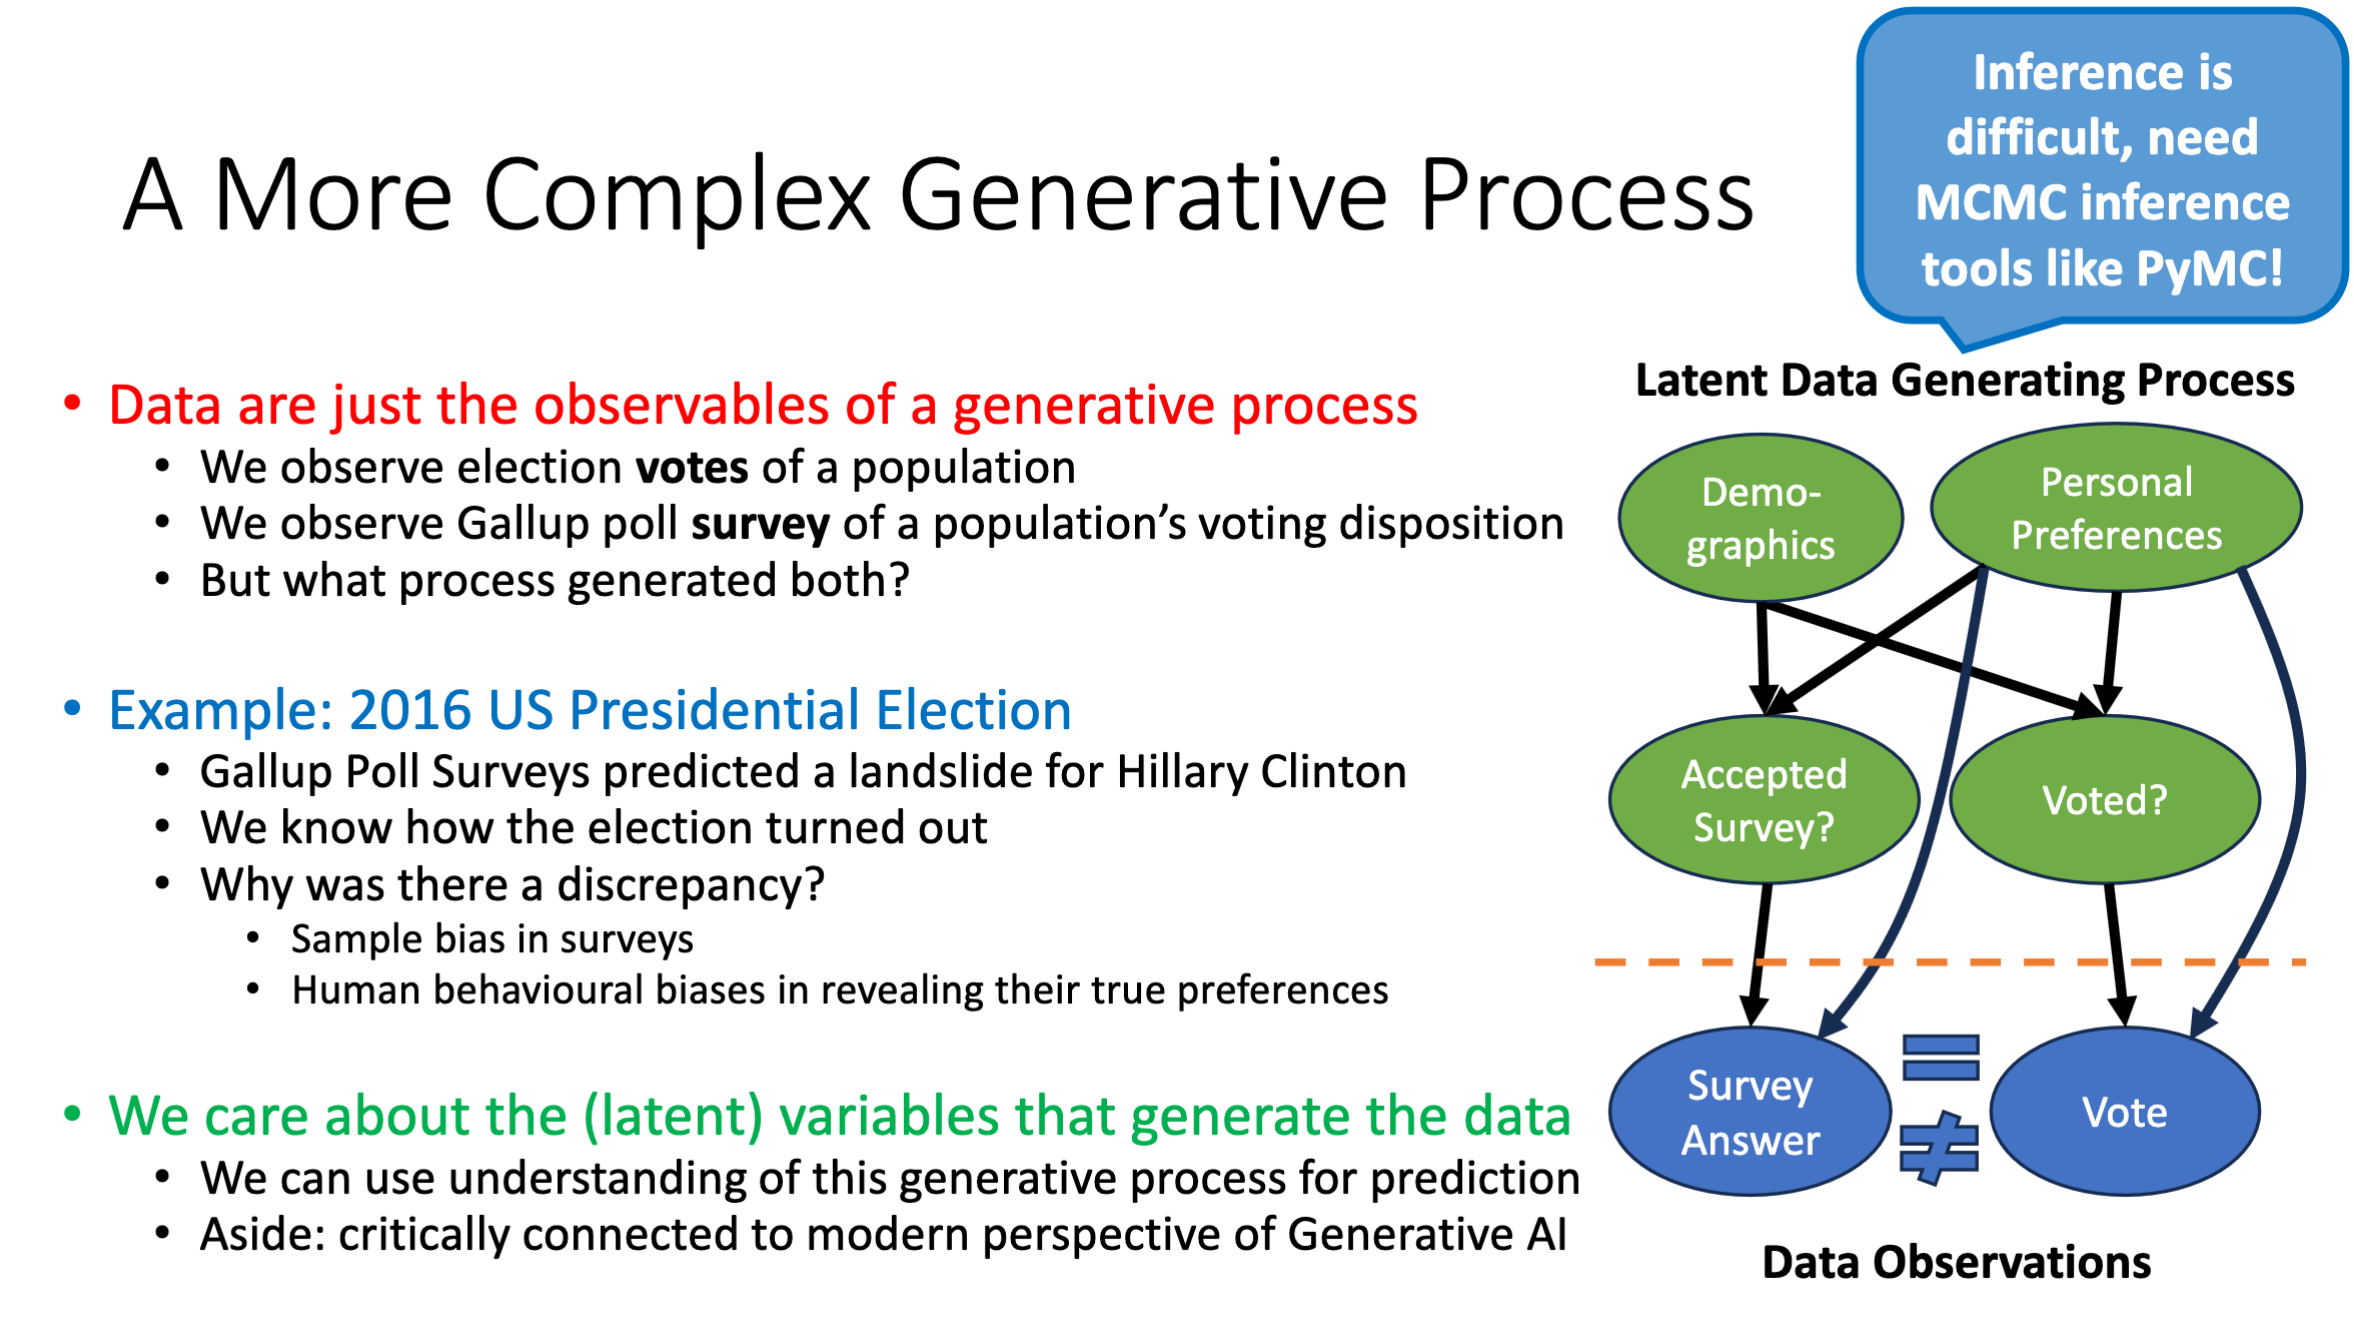
\includegraphics[width=\textwidth/2]{12.png}

Survey answer was inconsistent with the voting outcome. People who 
wanted to vote for Trump in 2016 did not admit it. You have the observed data,
so you can find the posterior distribution. This may reveal the percentage
of Trump voters who would answer the survey.

\end{document}